\documentclass{article}
\usepackage{graphicx}
\graphicspath{ {./images/} }
\begin{document}

%Header
\begin{flushleft}
Evan Wilcox\\
CS1200 Fall 2018\\
Homework 3\\
Due: Friday 10/05/18
\end{flushleft}

%Problems
\begin{enumerate}
    
    %1
    \item Show that $\rightarrow$ does not have the associative or 
    commutative laws.
    \begin{enumerate}
        
        %a
        \item $P \rightarrow (Q \rightarrow R)$ and $(P \rightarrow Q) \rightarrow R$ have different truth tables.\\
        \begin{tabular}{ |c|c|c|c|c| } 
            \hline
            $P$ & $Q$ & $R$ & $P \rightarrow (Q \rightarrow R)$ & $(P \rightarrow Q) \rightarrow R$\\ 
            \hline
            F & F & F & T & F\\ 
            \hline
            F & F & T & T & T\\ 
            \hline
            F & T & F & T & F\\ 
            \hline
            F & T & T & T & T\\ 
            \hline
            T & F & F & T & T\\ 
            \hline
            T & F & T & T & T\\ 
            \hline
            T & T & F & F & F\\ 
            \hline
            T & T & T & T & T\\ 
            \hline
        \end{tabular}

        %b
        \item $P \rightarrow Q$ and $Q \rightarrow P$ have different truth tables.\\
        \begin{tabular}{ |c|c|c|c|c| } 
            \hline
            $P$ & $Q$ & $P \rightarrow Q$ & $Q \rightarrow P$\\ 
            \hline
            F & F & T & T\\ 
            \hline
            F & T & T & F\\ 
            \hline
            T & F & F & T\\ 
            \hline
            T & T & T & T\\ 
            \hline
        \end{tabular}
    \end{enumerate}
    
    \newpage
    %2
    \item Verify the second DeMorgan's Law $\sim(P|Q) = \sim P\& \sim Q$ 
    manually using truth table.\\
    \vspace{1cm}
    \begin{tabular}{ |c|c|c|c|c|c|c| } 
        \hline
        $P$ & $Q$ & $\sim P$ & $\sim Q$ & $\sim(P|Q)$ & $\sim P\& \sim Q$\\ 
        \hline
        F & F & T & T & T & T\\ 
        \hline
        F & T & T & F & F & F\\ 
        \hline
        T & F & F & T & F & F\\ 
        \hline
        T & T & F & F & F & F\\ 
        \hline
    \end{tabular}

    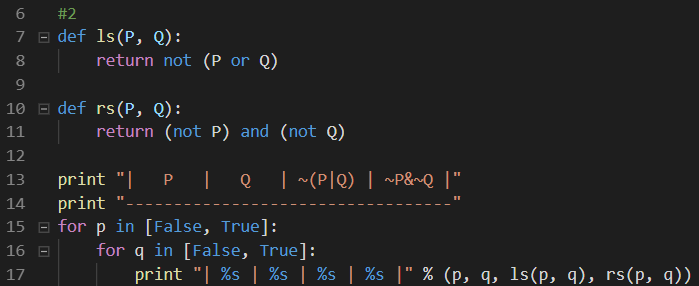
\includegraphics[scale=.75]{2a}

    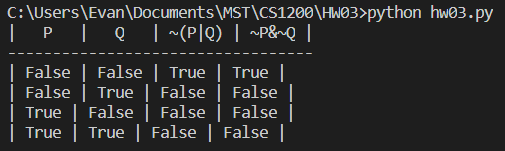
\includegraphics[scale=.75]{2b}

    \newpage
    %3
    \item 
    \begin{enumerate}
        
        %a
        \item Manually construct a truth table for $\sim(P\&Q \rightarrow R\& S)$\\
        \begin{tabular}{ |c|c|c|c|c|c|c|c| } 
            \hline
            $P$ & $Q$ & $R$ & $S$ & $P\& Q$ & $R \& S$ & $\rightarrow$ & $\sim(P\&Q \rightarrow R\& S)$\\ 
            \hline
            F & F & F & F & F & F & T & F\\ 
            \hline
            F & F & F & T & F & F & T & F\\ 
            \hline
            F & F & T & F & F & F & T & F\\ 
            \hline
            F & F & T & T & F & T & T & F\\ 
            \hline
            F & T & F & F & F & F & T & F\\ 
            \hline
            F & T & F & T & F & F & T & F\\ 
            \hline
            F & T & T & F & F & F & T & F\\ 
            \hline
            F & T & T & T & F & T & T & F\\ 
            \hline
            T & F & F & F & F & F & T & F\\ 
            \hline
            T & F & F & T & F & F & T & F\\ 
            \hline
            T & F & T & F & F & F & T & F\\ 
            \hline
            T & F & T & T & F & T & T & F\\ 
            \hline
            T & T & F & F & T & F & F & T\\ 
            \hline
            T & T & F & T & T & F & F & T\\ 
            \hline
            T & T & T & F & T & F & F & T\\ 
            \hline
            T & T & T & T & T & T & T & F\\ 
            \hline

        \end{tabular}
        
        %b
        \item Find the disjunctive normal form of $\sim(P\&Q \rightarrow R\& S)$.\\
        $$(P\& Q\& \sim R) | (P \& Q \& \sim S)$$
    \end{enumerate}

    \newpage
    %4
    \item Let $G(A,B,C)$ be the function: $$B\&A|C\&C\leftarrow B\&B\rightarrow B!=A|C$$
    \begin{enumerate}
        
        %a
        \item Completely parenthesize the above expression for G.
        $$(((((B\&A)|(C\&C))\leftarrow (B\&B))\rightarrow B)!=(A|C))$$
        
        %b
        \item Create a truth table for G.\\
        \begin{tabular}{ |c|c|c|c|c|c|c|c|c|c|c|c| } 
            \hline
            $A$ & $B$ & $C$ & $B\&A$ & $|$ & $C\&C$ & $\leftarrow$ & $B\&B$ & $\rightarrow B$ & $!=$ & $A|C$ & $G$\\ 
            \hline
            F & F & F & F & F & F & T & F & F & F & F & F\\ 
            \hline
            F & F & T & F & T & T & T & F & F & T & T & T\\ 
            \hline
            F & T & F & F & F & F & F & T & T & T & F & T\\ 
            \hline
            F & T & T & F & T & T & T & T & T & F & T & F\\ 
            \hline
            T & F & F & F & F & F & T & F & F & T & T & T\\ 
            \hline
            T & F & T & F & T & T & T & F & F & T & T & T\\ 
            \hline
            T & T & F & T & T & F & T & T & T & F & T & F\\ 
            \hline
            T & T & T & T & T & T & T & T & T & F & T & F\\ 
            \hline
        \end{tabular}

        %c
        \item Express G in disjunctive normal form.
        $$(\sim A \& \sim C) | \sim B$$

        %d
        \item Draw a circuit that uses $\&$, $\mid$, and $\sim$ gates to 
        compute G.\\
        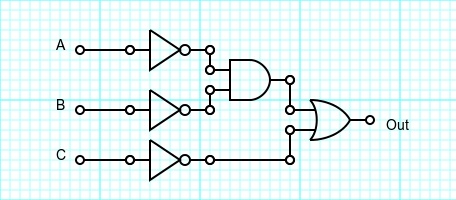
\includegraphics[scale=.9]{4d}
    \end{enumerate}
    
    \newpage
    %5
    \item Represent the function $P!=(Q!=R)$ using NOT, AND and OR gates.\\
    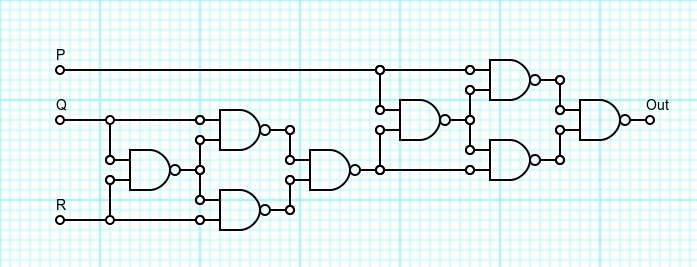
\includegraphics[scale=.9]{5}

    %6
    \item Design a circuit for three switches that turns a light on only if 
    at least two of the three switches are on.\\
    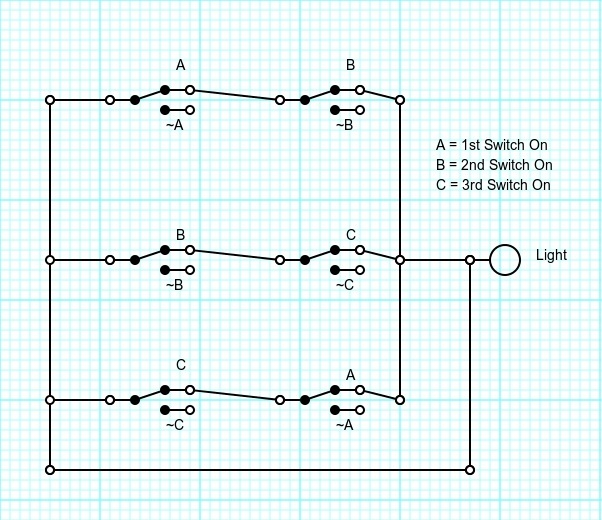
\includegraphics[scale=1]{6}


\end{enumerate}

\end{document}